\documentclass[a4paper]{article}

\usepackage[czech]{babel}
\usepackage[utf8]{inputenc}
\usepackage{amsmath}
\usepackage{graphicx}
\usepackage{url}

\title{Řešení optimalizační úlohy Capacitated VRP pomocí genetického algoritmu v~paralelním prostředí}

\author{Jan Sedlák}

\date{\today}

\begin{document}
\maketitle

\section{Úvod}

Vehicle Routing Problem, neboli \emph{VRP}, popisuje optimalizační úlohu minimalizace cesty v~grafu~\cite{dantzig}. Tento graf si můžeme představit jako systém s~několika místy a vozidly. Vozidla začínají a končí svoji trasu v~jednom místě. Všechna ostatní místa musí být navštívena právě jednou - úkolem je naleznout takové rozvržení míst mezi jednotlivá vozidla a takové pořadí těchto míst na trase vozidla, aby souhrnná uražená vzdálenost všech vozidel byla co nejmenší. Varianta Capacitated pak přidává ke každému místu hodnotu - \emph{požadavek} - a u~vozidel specifikuje jejich kapacitu. Součet požadavků na trase nesmí překročit kapacitu vozidla.

Jako analogii ve skutečném světě si můžeme představit rozvoz zboží. Zboží se rozváží z~centrály zákazníkům po městě. K~dispozici máme několik vozů s~konkrétní kapacitou. Naším cílem je rozvézt zboží mezi všechny zákazníky tak, abychom uspokojili poptávku každého zákazníka a při tom minimalizovali náklady na pohonné hmoty.

VRP je NP-těžký problém~\cite{yucenur}, tudíž není možno zajistit, že jeho optimální řešení nalezneme pouhým prohledáváním stavového prostoru do šířky nebo hloubky v~polynomiálním čase. Tyto problémy se také nazývají \emph{kombinatorické optimalizace} a jejich optimální hodnoty často nejsme schopni nalézt přímo. V~tom případě používáme různé heuristické metody, které jsou schopny se k~optimálnímu řešení přiblížit. Mezi takovéto metody patří například optimalizace mravenčí kolonií, simulované žíhání či genetický algoritmus.

Tato práce se zabývá řešením optimalizace úlohy Vehicle Routing Problem, varianty Capacitated, za pomocí genetického algoritmu. Jsou zkoumány mož\-nos\-ti implementace tohoto algoritmu v~paralelním prostředí a vliv proměnných genetického algoritmu (jako je například velikost populace či míra mutace) na rychlost konvergence genetického algoritmu a kvalitu řešení. Experimentální ověření proběhlo na dvou úlohách převzatých ze stránek skupiny NEO z~University of Malaga.

Odbornou konzultaci k~této práci ohledně některých rysů genetického algoritmu poskytl Dr.\ Ing.\ Petr Peringer.

\section{Rozbor tématu a použitých metod}

Řešením úlohy VRP rozumíme nalezení způsobu, jak obsloužit určitý počet zákazníků určitým počtem vozidel s~co nejmenší uraženou vzdáleností~\cite{neo}.

\subsection{Úloha Vehicle Routing Problem}

Formálně je úloha CVRP~\cite{neo} zadaná jako graf $G(V,E)$, kde:

\begin{itemize}
\item $V = \left\{v_0,v_1,\dots,v_n\right\}$ je množina vrcholů, kde $v_0$ reprezentuje výchozí bod (centrálu) a
\item $E = \left\{(v_i,v_j)|v_i,v_j\in V; i \neq j\right\}$ je množina hran, spojující tyto vrcholy.
\end{itemize}

\noindent Dále definujeme:

\begin{itemize}
\item $V' = V\setminus \left\{x_0\right\}$ je množina $n$ měst,
\item $C$ je matice vzdáleností mezi vrcholy,
\item $d$ je vektor požadavků v~jednotlivých vrcholech,
\item $R_i$ je cesta vozu $i$,
\item $m$ je počet (identických) vozidel a
\item $Q$ je kapacita každého vozidla.
\end{itemize}

\noindent Řešením Capacitated CVRP je potom:

\begin{itemize}
\item rozdělení $V'$ na $R_1,\dots,R_m$ a
\item permutace $\sigma_i$ množiny $R_i$, udávající pořadí obsluhy zákazníků na trase $i$,
\end{itemize}

\noindent přičemž žádné vozidlo nepřekročí limit své kapacity, čili $\sum\limits_{i=1}^{m}d_i\leq Q$~\cite{cneo}. Cenu $C$ řešení $Ri$ určíme jako $C(Ri)=\sum\limits_{i=0}^m c_{i,i+1}$.

Naším úkolem je minimalizovat cenu, snažíme se tedy nalézt takové řešení $R$, že $\sum\limits_{i=1}^m C(R_i)$ je co nejmenší.

\subsection{Genetický algoritmus}
Genetický algoritmus je programový model genetického vývoje~\cite{sfc}, který je použit pro přiblížení se k~optimálnímu řešení dané úlohy. Každé řešení problému - jedinec - je reprezentované \emph{chromozomem}. Algoritmus udržuje určitý počet jedinců, \emph{populaci}, a v~každém kroku několik z~nich prokříží, čímž vznikne nová \emph{generace}. Genetický algoritmus také musí obsahovat hodnotící funkci, takzvanou \emph{fitness}. Fitness funkce musí být schopna u~každého řešení určit, jak je kvalitní, čili jak je vzdálené od optimálního řešení. Aby při řešení problému genetickým algoritmem nedošlo k~zastavení v~lokálním maximu, musí docházet k~\emph{mutacím}. Mutace je náhodný děj, který s~určitou pravděpodobností provede drobnou změnu v~chromozomu jedince. V~permutačních problémech je nejlepším způsobem mutace prohození pozice dvou hodnot~\cite{adal}.

Pokud je zvoleno vhodné křížení a vhodná reprezentace jedince a systém se nechová chaoticky, křížení dvou jedinců s~vysokou hodnotou fitness může často vést k~tomu, že jedinec převezme tu lepší část řešení s~obou rodičů. Je však nutné pečlivě vybrat algoritmy pro výběr rodičů, křížení a mutaci jedinců.

\subsubsection{Způsob výběru rodičů}
Prvním krokem při křížení jedinců je výběr rodičů. Je důležité, aby hodnota fitness funkce odpovídala pravděpodobnosti výběru jedince pro křížení~\cite{sfc}. Tím se zajistí, že pro křížení budou častěji vybírání jedinci s~vyšší hodnotou fitness funkce a zároveň, protože pro výběr mají šanci i jedinci s~nižší hodnotou fitness funkce, algoritmus nebude mít tendenci uváznout v~lokálním maximu. Samotný výběr rodičů může být implementován několika způsoby:

\begin{description}
\item[výběr elity] způsobí, že pro křížení je vybráno pouze prvních $N$ jedinců s~nejlepším fitness,
\item[výběr pomocí rulety] znamená, že každý jedinec získá výseč rulety, poměrově odpovídající hodnotě jeho fitness. Následně je vygenerováno náhodné číslo, které je převedeno na odpovídající místo v~ruletě a vybraný je jedinec, do jehož výseče toto místo spadá, nebo
\item[algoritmus turnaje] při kterém je z~populace získán náhodný vzorek jedinců a jako rodič je vybraný ten s~nejvyšší hodnotou fitness.
\end{description}

\subsubsection{Způsob křížení}
Jakmile jsou vybráni jedinci jako rodiče, přichází na řadu jejich křížení. Vý\-sled\-kem křížení je jeden nebo více jedinců, přičemž každý nese část genetické informace od každého svého rodiče. Vhodnost různých způsobů křížení závisí na reprezentaci chromozomu a také na řešeném problému. Mezi možné způsoby křížení patří:

\begin{description}
\item[jednobodové křížení] znamená, že je v~chromozomu zvolen jeden náhodný bod a potomek získá první část genetické informace od jednoho rodiče a zbytek od druhého,
\item[vícebodové křížení] funguje v~principu stejně jako jednobodové, pouze na dalším náhodně zvoleném bodě bude potomek opět brát informaci z~prv\-ní\-ho rodiče,
\item[uniformní křížení] znamená, že se každý prvek chromozomu přenese se stejnou pravděpodobností od jednoho nebo druhého rodiče,
\item[aritmetické křížení] je vhodné, pokud jsou prvky chromozomu reálná čísla. Výsledný potomek pak může brát hodnoty obou rodičů zaráz, vždy s~ur\-či\-tou vahou.
\end{description}

VRP patří mezi problémy, jehož nejjednodušší reprezentace v~chromozomu je permutace míst. Pokud bychom však použili nějaký z~výše uvedených způsobů křížení, často by vznikaly neplatné reprezentace. Například zkřížením chromozomu [A, B, C, D] a [D, C, B, A] pro nějaký problém může jednobodovým křížením vzniknout chromozom [A, B, B, A], který však v~permutační úloze není platný. Je proto nutné použít křížení, které je pro permutační optimalizační problémy uzpůsobeno~\cite{sfc}. Jedním z~těchto křížení je jednobodové křížení s~použitím indexové tabulky. Chromozom je neprve převeden do \emph{indexového chromozomu}, ten je zkřížen jednobodovým křížením a výsledek je převeden zpět.

Křížení více jedinců však není v~genetických algoritmech nutné, například pokud charakter úlohy a reprezentace chromozomu zapříčiní, že potomek není po prokřížení podobný ani jednomu svému rodiči. Při řešení VRP je možné křížení více jedinců zanedbat a nové jedince vytvářet pouze na základě jednoho stávajícího, pomocí mutace či různých heuristik~\cite{masum}.

\subsection{Paralelní zpracování}
Jasným trendem několika posledních let je zvyšující se počet procesorových jader v~systému~\cite{sekanina}. Aby však bylo možné tyto multiprocesorové systémy využít, jsou často potřeba netriviální úpravy algoritmů.

Řešením může být použití takového programovacího jazyka, který je na implementaci paralelního řešení navrhnut a uzpůsoben. Jedním z~těchto jazyků je funkcionální jazyk Erlang. Erlang obsahuje konstrukt pro spuštění procesu a jeho komunikaci s~okolím. Nejedná se však o~procesy v~pravém slova smyslu - jde o~tzv.\ \emph{green thread}, čili vlákna, které si běhové prostředí řídí samo. Díky tomu je běhové prostředí Erlangu schopno velice rychle spustit a řídit větší množství procesů~\cite{armstrong}, řádově statisíce až miliony.

VM Erlangu spustí na každém procesoru plánovač běhu procesů, tudíž správ\-ně napsaná aplikace v~Erlangu je schopna často využít plný výkon vícejádrového počítače.

\section{Koncepce optimalizačního programu pro ú\-lo\-hu CVRP}
Pro chování jednotlivých fází genetického algoritmu je důležité zvolit vhodnou reprezentaci chromozomu. Jelikož CVRP je permutační optimalizační úloha, chromozom může být reprezentován jako permutace seznamu měst. Každá po\-lož\-ka označuje ná\-sle\-du\-jící město, do kterého se má vozidlo vydat. Centrála je na začátek a konec cesty přidána automaticky.

Protože chromozom musí nést i informaci o~rozdělení tras mezi jednotlivá vozidla, finální podoba chromozomu je vektor vektorů, kde jednotlivé vnořené vektory můžou být různě dlouhé a reprezentují $R_i$ cesty jednotlivých vozidel.

Fitness funkce je v~kontextu VRP předem jasná - jedná se o~součet uražené vzdálenosti. Dle~\cite{cneo} je vhodné jedince s~překročenou kapacitou z~populace ne\-vy\-řa\-zo\-vat, pouze tento fakt zohledit v~hodnotící funkci. Finální podoba fitness funkce je tedy:

\[f(x) = soucet\_vzdalenosti(x) + \lambda*pres\_kapacitu(x)\]

\noindent kde $soucet\_vzdalenosti(x)$ je funkce, která pro zadaný chromozom spočítá kompletní uraženou vzdálenost, $pres\_kapacitu(x)$ vrací počet jednotek překročené kapacity a $\lambda$ je koeficient pokuty za překročení kapacity. Důležité je, že takováto podoba fitness funkce znamená, že kvalitnější řešení jsou ty s~menším score. Hodnotu fitness problému se tudíž nebudeme snažit maximalizovat, ale minimalizovat. Na princip fungování genetického algoritmu to však nemá vliv.

Pro křížení bylo vybráno jednobodové křížení s~využitím indexové tabulky a pro výběr rodičů algoritmus turnaje. Po křížení vzniknou dva potomci. První potomek přebere rozdělení měst mezi vozidla od prvního rodiče, druhý potomek od druhého rodiče. Při mutaci dochází k~prohození pozice dvou měst a to buď v~rámci cesty jednoho vozidla, nebo prohození měst mezi vozidly. Může také dojít ke kompletnímu odebrání města z~trasy jednoho vozidla a jeho přidání do trasy jiného.

V~průběhu genetického algoritmu zůstává počet jedinců v~populaci neměnný. V~každé generaci se vyberou dvě třetiny jedinců pro křížení, přičemž jeden jedinec může být vybrán několikrát. Nejlepší třetina populace zůstane mezi generacemi zachována jako elita, zbylé dvě třetiny jsou nahrazeny potomky z~křížení. Z~každého jednoho křížení vzniknou dva potomci, oba jsou se zadanou pravděpodobností mutováni.

\section{Implementace}
Jak již bylo řečeno, optimalizační program je implementován ve funkcionálním jazyce v~paralelním prostředí. Procesy v~jazyce Erlang neobsahují sdílenou paměť. Jejich komunikace je zajištěna pomocí asynchronního zasílání zpráv, jedná se de fakto o~multiagentní systém. Hlavní proces, {\tt main}, se stará o~načtení vstupního souboru ve formátu TSPLIB, vygenerování počáteční populace a vytvoření procesu pro každého jedince v~populaci. Proces spočítá hodnotu fitness funkce svého chromozomu. {\tt main} následně z~těchto procesů vytvoří strom - každému procesu zašle zprávu, obsahující PID jeho levého a pravého potomka. Nakonec vytvoří poslední proces, který se stará o~samotný průběh genetického algoritmu.

V~každé iteraci genetického algoritmu pošle řídící proces prvnímu procesu zprávu, požadavek o~vzestupně seřazený seznam fitness funkcí všech jedinců spolu s~identifikátory procesů PID. Každý list zašle požadavek svým potomkům a po přijetí seznamů z~obou podstromů tyto seznamy spojí (\emph{merge}), vloží do něj svoji hodnotu fitness a celý výsledný seznam odešle nadřazenému procesu. Jakmile řídící proces získá seřazený seznam všech hodnot fitness, vytvoří nové procesy {\tt tournament\_selector} pro křížení. Každý tento proces vygeneruje $N$ náhodných čísel, z~nich vezme dvě nejmenší a použije je jako index do seřazeného seznamu fitness, tím je simulován algoritmus turnaje. Od procesů s~danou fitness získá jejich reprezentaci, nad tou provede křížení a případnou mutaci a výsledek zašle řídícímu procesu. Řídící proces tyto nově vzniklé chromozomy zašle nejhorším dvěma třetinám procesů podle seznamu výsledků fitness funkcí a tím je ukončen jeden krok genetického algoritmu.

Pro měření zrychlení paralelního řešení byla naprogramována také verze bez paralelismu, která pro výpočet používá funkce pro práci se seznamy. Paralelní verze se nachází v~souboru {\tt vrp.erl}, neparalelní verze v~sou\-bo\-ru {\tt vrpserial.erl}.

\section{Experimentální ověření optimalizátoru}

Experimenty chceme ověřit, že navrhnutý a implementovaný optimalizátor do\-ká\-že pomocí genetického algoritmu řešit zadanou optimalizační úlohu CVRP, zkoumat vlastnosti systému v~závislosti na použitých proměnných jako je velikost populace, míra mutace a velikost skupiny vybraných jedinců pro křížení turnajem a dále dokázat, že paralelní řešení zrychlí běh úlohy.

\subsection{Vliv proměnných na kvalitu řešení a rychlost konvergence}

Pro experimentální ověření bylo provedeno 80 experimentů, čili spuštění optimalizátoru pro různé vstupní proměnné. Je však důležité si uvědomit, že genetický algoritmus je založen na prvku náhody. Proto je vhodné spíše sledovat trend vývoje kvality řešení, než absolutně spoléhat na získané hodnoty. Všechny grafy v~této sekci byly upraveny tak, aby osa $x$ zobrazovala část od začátku po ustálení a osa $y$ zobrazovala rozsah od hodnoty pod optimálním řešením po hodnotu, ve které se jednotlivé řešení začnou rozcházet.

První zadání je úloha A-n32-k5.vrp z~datasetu Augeral a kol. Úloha obsahuje 32 měst, u~každého známe jeho souřadnice a požadavek. Cena přechodu mezi dvěma městy je určena euklidovskou vzdáleností těchto dvou měst. Optimální hodnota ceny průchodu všemi městy je 784.

Nejprve prozkoumejme závislost velikosti populace na rychlosti konvergence a kvalitě výsledného řešení. Měření probíhalo pro míru mutace 75 \% a pro 5 jedinců na jeden turnaj (důvod volby těchto konstant nám bude jasný z~ná\-sle\-du\-jí\-cích grafů). Výsledný graf je vidět na obrázku~\ref{fig:populace}. Jak je z~grafu zřejmé, pro zadané konstanty je lepší vyšší počet jedinců. Jakmile počet jedinců přesáhne určitou hranici, která je nutná pro dostatečnou rozmanitost, neexistuje horní hranice ideálního počtu jedinců. Jak vyplývá z~grafů~\ref{fig:padesat} a~\ref{fig:tisic}, může být počet padesáti jedinců v~populaci velice často nedostatečný. Musíme ale také myslet na to, že větší počet jedinců znamená delší výpočet, jak bude zřejmé z~dalších experimentů. Menší počet jedinců má také větší tendence uváznout v~lokálním minimu.

\begin{figure}
\centering
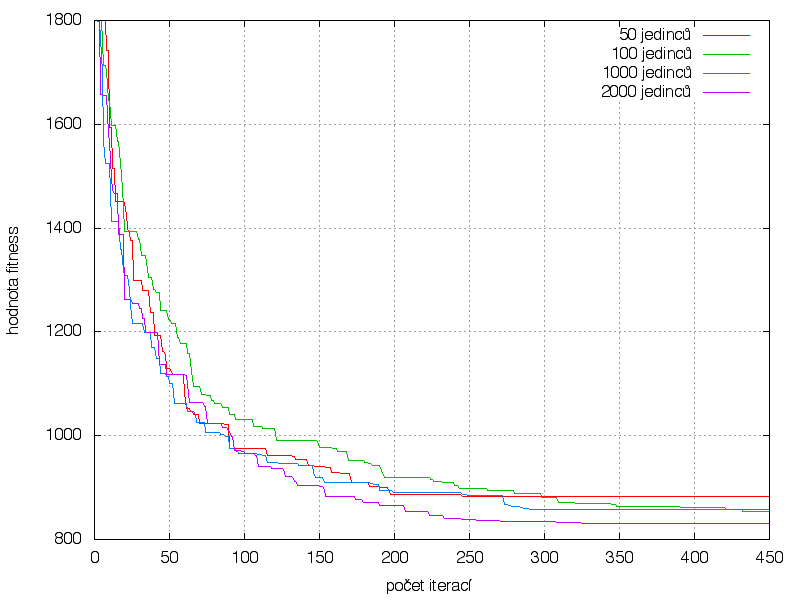
\includegraphics[width=\textwidth]{populace.png}
\caption{Závislost počtu jedinců na kvalitě výsledného řešení u~problému A-n32 pro 32 měst a 5 vozidel\label{fig:populace}}
\end{figure}

\begin{figure}
\centering
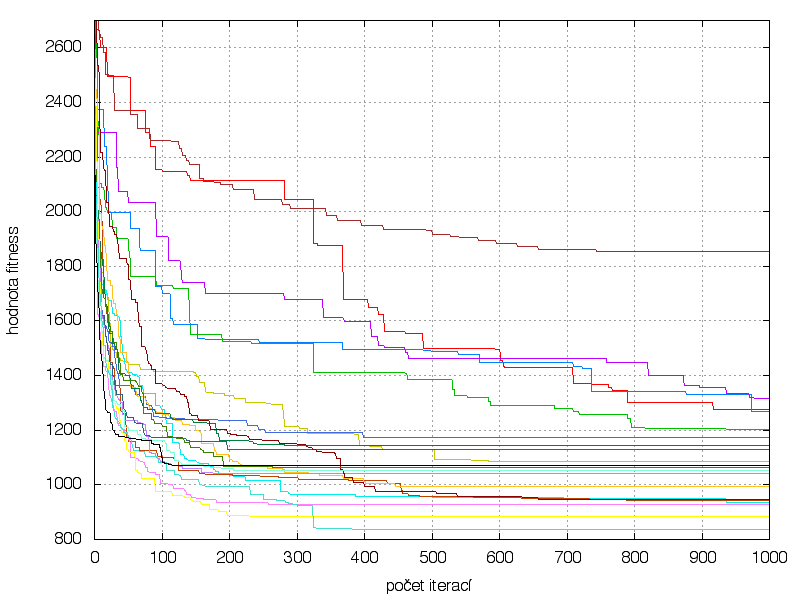
\includegraphics[width=\textwidth]{padesat.png}
\caption{Orientační výsledky pro populaci s~50 jedinci problému A-n32 pro 32 měst a 5 vozidel\label{fig:padesat}}
\end{figure}

\begin{figure}
\centering
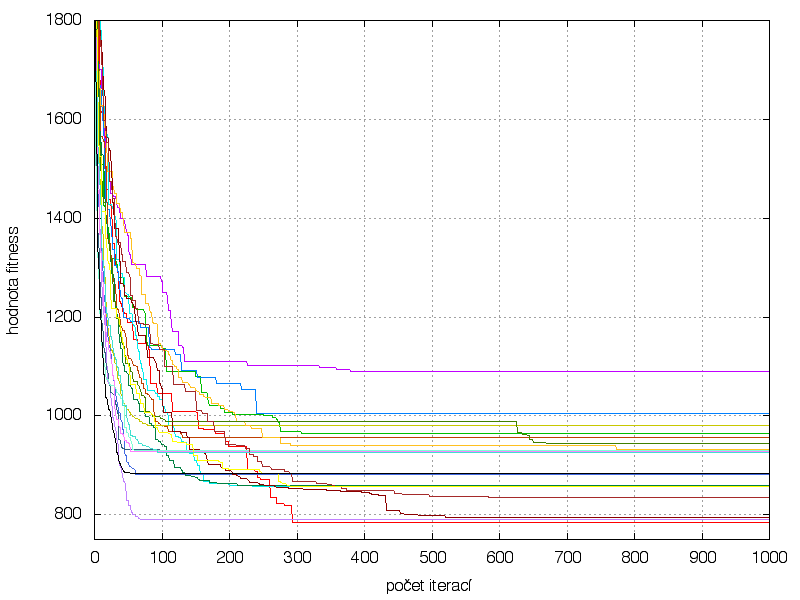
\includegraphics[width=\textwidth]{tisic.png}
\caption{Orientační výsledky pro populaci s~1000 jedinci problému A-n32 pro 32 měst a 5 vozidel\label{fig:tisic}}
\end{figure}

Dále budeme zkoumat závislost míry mutace na kvalitu řešení. Ačkoliv je doporučováno, aby míra mutace byla velice malá~\cite{sfc}, výsledky měření mluví o~opaku. Jak je vidět na obrázku~\ref{fig:mutace}, vyšší míra mutace má za následek kvalitnější výsledky. Velmi malá míra mutace totiž vede k~tendenci uváznutí v~lokálním minimu. Výsledek po křížení dvou stejných jedinců jsou opět dva jedinci, stejní jako jejich rodiče, což má za následek zaplnění celé populace stejnými jedinci.

\begin{figure}
\centering
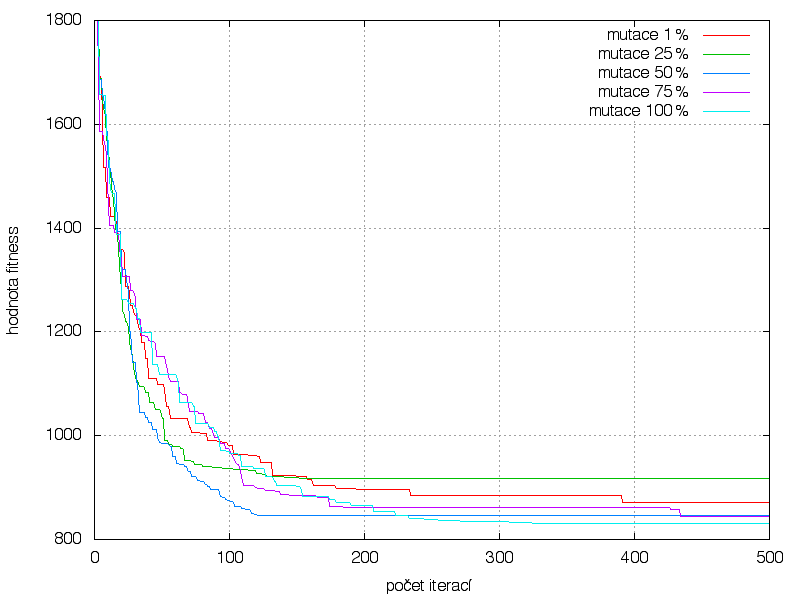
\includegraphics[width=\textwidth]{mutace.png}
\caption{Závislost míry mutace na kvalitě výsledného řešení u~problému A-n32 pro 32 měst a 5 vozidel\label{fig:mutace}}
\end{figure}

Zajímavý je vliv počtu jedinců v~jedné skupině při turnaji. Jak je vidět na obrázku~\ref{fig:turnaj}, vyšší počet jedinců znamená vyšší pravděpodobnost, že se do skupiny dostane elita. Důsledkem je malá diverzita populace a po rychlé konvergenci vede k~uváznutí v~lokálním minimu.

\begin{figure}
\centering
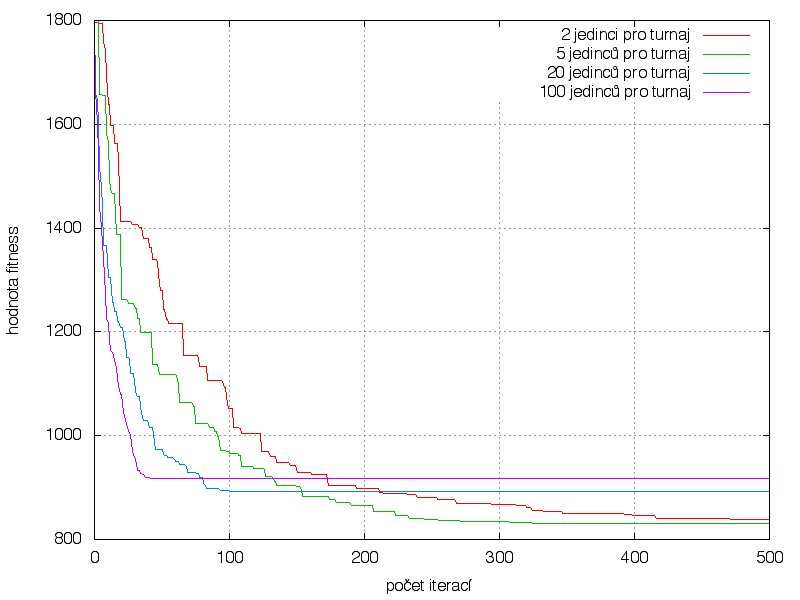
\includegraphics[width=\textwidth]{turnaj.png}
\caption{Závislost počtu jedinců při výběru turnajem na kvalitě výsledného řešení u~problému A-n32 pro 32 měst a 5 vozidel\label{fig:turnaj}}
\end{figure}

Na obrázku~\ref{fig:best} jsou zobrazena nejlepší dosažená řešení. Je důležité určit vhodný koeficient pokuty za překročení kapacity. Pokud je tento koeficient příliš malý, algoritmus nedbá na překročení kapacity a výsledkem je neplatné řešení. Pokud je tento koeficient příliš velký, algoritmus méně `riskuje', což má za následek brzké zahození řešení, které je blízko optimálnímu, ale má překročenou kapacitu, čili vede k~uváznutí v~lokálním minimu. Všechny tyto experimenty byly testovány v~koeficientem 10.

\begin{figure}
\centering
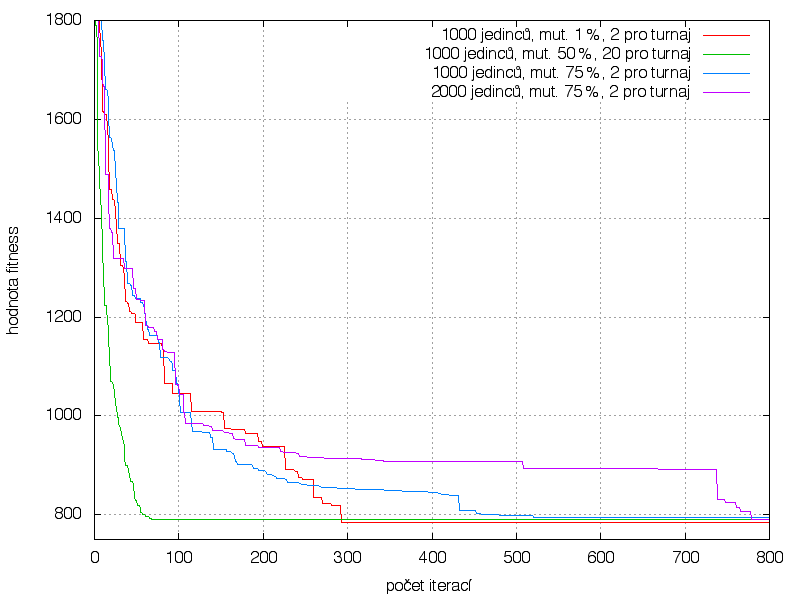
\includegraphics[width=\textwidth]{best.png}
\caption{Nejlepší výsledky u~problému A-n32 pro 32 měst a 5 vozidel\label{fig:best}}
\end{figure}

Nakonec jsou na obrázku~\ref{fig:ntrisedm} představeny výsledky pro úlohu A-n37-k6.vrp pro systém z~37 městy a 6 vozidly. Graf zobrazuje souhrnně rychlost konvergence a kvalitu výsledného řešení pro mutaci 1 \%, 75 \% a 100 \%.

Pro zajímavost je na obrázku~\ref{fig:cesta} vizualizováno jedno z~řešeních úlohy A-n32.

\begin{figure}
\centering
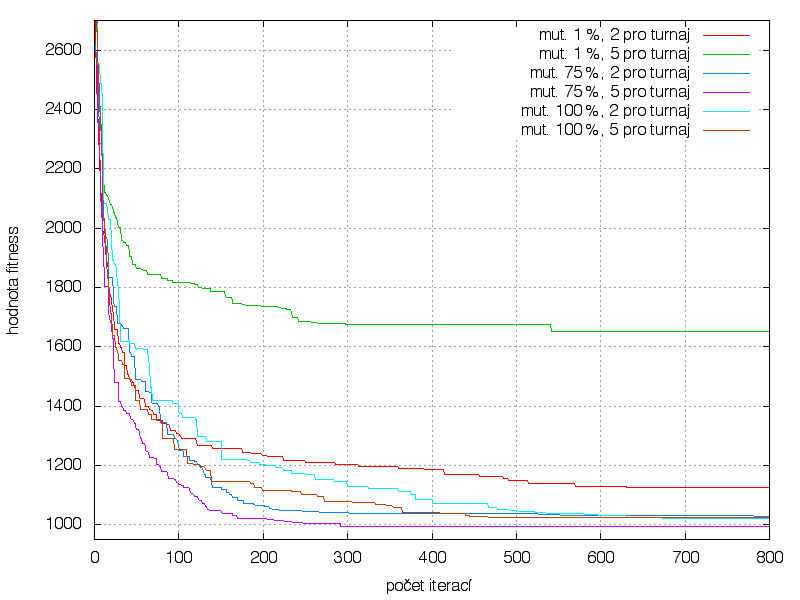
\includegraphics[width=\textwidth]{ntrisedm.png}
\caption{Výsledky pro populaci s~2000 jedinci problému A-n37 pro 37 měst a 6 vozidel\label{fig:ntrisedm}}
\end{figure}

\begin{figure}
\centering
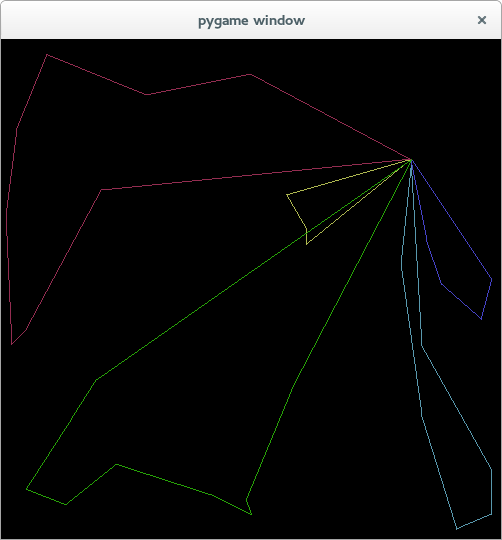
\includegraphics[width=\textwidth]{cesta.png}
\caption{Vizualizace jednoho z~nalezených řešení problému A-n37\label{fig:cesta}}
\end{figure}

\subsection{Ověření kvality paralelního řešení}

Pro ověření kvality paralelní řešení nás zajímá doba výpočtu řešení úlohy A-n32-k5.vrp pro proměnný počet jedinců. Ověření probíhalo na systému s~2jádrovým procesorem Intel Core i5 s~technologií hyperthreading, čili systém má k~dispozici 4 virtuální thready. Jak vyplývá z grafu~\ref{fig:procesory}, paralelní řešení skutečně zrychlí výpočet úlohy.

\begin{figure}
\centering
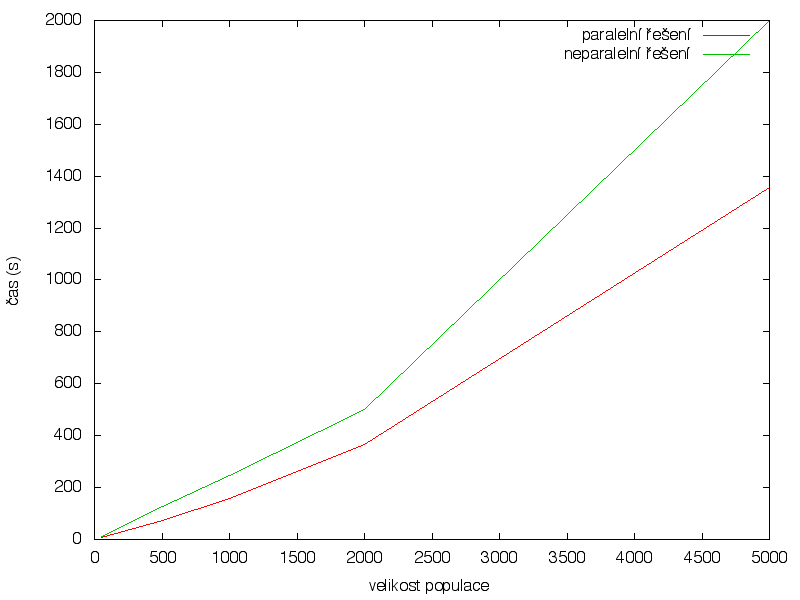
\includegraphics[width=\textwidth]{procesory.png}
\caption{Graf závislosti počtu jedinců na době výpočtu pro paralelní a neparalelní řešení\label{fig:procesory}}
\end{figure}

\subsection{Závěry experimentů}
Bylo provedeno 80 experimentů s~úlohou A-n32 a 18 experimentů s~úlohou A-n37 při různých parametrech genetického algoritmu. Pro přesnější výsledky by bylo vhodné každý z~těchto experimentů provést opakovaně a sledovat například i průměrnou kvalitu jednoho nastavení parametrů.

\section{Závěr a zhodnocení výsledků}
V~této práci byl představen popis a implementace optimalizačního programu pro úlohu CVRP pomocí genetických algoritmů a to v~paralelním prostředí. Experimentálně bylo zjištěno, že v~navrhnutém řešení problému vede vysoká míra mutace k~lepším řešením. To je zřejmě způsobeno vybraným způsobem mutace, ta zde může do určité míry nahrazovat křížení.

Dále bylo zjištěno, že pro rychlejší konvergenci a kvalitnější výsledné řešení je vhodný větší počet jedinců v~populaci. Zajistí se tak větší variabilita testovaných řešení, avšak se vzrůstajícím počtem jedinců v~populaci roste doba výpočtu genetického algoritmu.

Experimentálně bylo ověřeno, že navrhnuté paralelní řešení na stroji s~více jádry procesoru zrychlí výpočet genetického algoritmu zhruba o~třetinu. To může být způsobeno tím, že ačkoliv velká část výpočtu probíhá paralelně, tak v~každé generaci musí řídící proces získat výsledky všech fitness funkcí a následně je předat ostatním. Větší míra zrychlení by zřejmě byla možná pokud by v~programu nenastalo, že ostatní procesy čekají na dokončení výpočtu jednoho jediného procesoru.

\begin{thebibliography}{9}
\bibitem{dantzig}
Dantzig, George B.; Ramser, John H.,
\emph{The truck dispatching problem}.
Management science, 1959.
\bibitem{yucenur}
Yucenur, G. N.; Demirel, N.C.,
\emph{A~new geometric shape-based genetic clustering algorithm for the multi-depot vehicle routing problem}.
Expert Systems With Applications, 2011
\bibitem{neo}
Networking and Emerging Optimization, Deptarment of LCC from the University of Malaga,
\emph{Vehicle Routing Problem}.
\url{http://neo.lcc.uma.es/vrp/vehicle-routing-problem/}.
\bibitem{cneo}
Networking and Emerging Optimization, Deptarment of LCC from the University of Malaga,
\emph{Capacitated VRP}.
\url{http://neo.lcc.uma.es/vrp/vrp-flavors/capacitated-vrp/}
\bibitem{sfc}
Zbořil, František V., doc. Ing., CSc.,
\emph{Genetické algoritmy}.
doprovodné materiály k~předmětu SFC,
2014.
\bibitem{adal}
Áslaug Sóley Bjarnadóttir,
\emph{Solving the Vehicle Routing Problem with Genetic Algorithms}.
Technical University of Denmark,
2004.
\bibitem{masum}
Masum, Abdul Kadar Muhammad, et al.,
\emph{Solving the Vehicle Routing Problem using Genetic Algorithm}.
International Journal of Advanced Computer Science \& Applications 2.7,
2011.
\bibitem{sekanina}
Sekanina, L, prof. Ing., Ph.D.,
\emph{Úvod do paralelních systémů}.
doprovodné materiály k~předmětu INP,
2013.
\bibitem{armstrong}
Armstrong, J.,
\emph{Programming Erlang: Software for a Concurrent World}.
Pragmatic Programmers,
2013.
\end{thebibliography}
\end{document}